\documentclass[10pt]{article}
\usepackage{longtable}
\usepackage{float}
\usepackage{wrapfig}
\usepackage{rotating}
\usepackage[normalem]{ulem}
\usepackage{amsmath}
\usepackage{textcomp}
\usepackage{marvosym}
\usepackage{wasysym}
\usepackage{amssymb}
\usepackage{hyperref}
\usepackage{color,soul} % for highlighting
\usepackage{graphicx}
\graphicspath{{/Users/benjaminbass/seacloud/class/earthMaterials/mineralSheets/tectosilicates/microcline/images/}}

\usepackage{frame,color}
\usepackage{framed}
\usepackage{minibox}

% \usepackage[T1]{fontenc}
% \usepackage{tilting} %bring title up
% \setlength{\droptitle}{-10cm}

\usepackage[version=3]{mhchem}
% How to Use MChem
% \ce{SO4^2-}
% \ce{^{227}_{90}Th+}
% \ce{A\bond{-}B\bond{=}C\bond{#}D}
% \ce{CO2 + C -> 2CO}
% \ce{SO4^2- + Ba^2+ -> BaSO4 v}


\author{Benjamin Bass}
\date{24 February 2016}
\title{\vspace{-2.0cm}Microcline} %bring title up temporary Fix

\begin{document}

\maketitle

% \framebox{Use frameboxes until figure out alignmen}

\begin{center}
  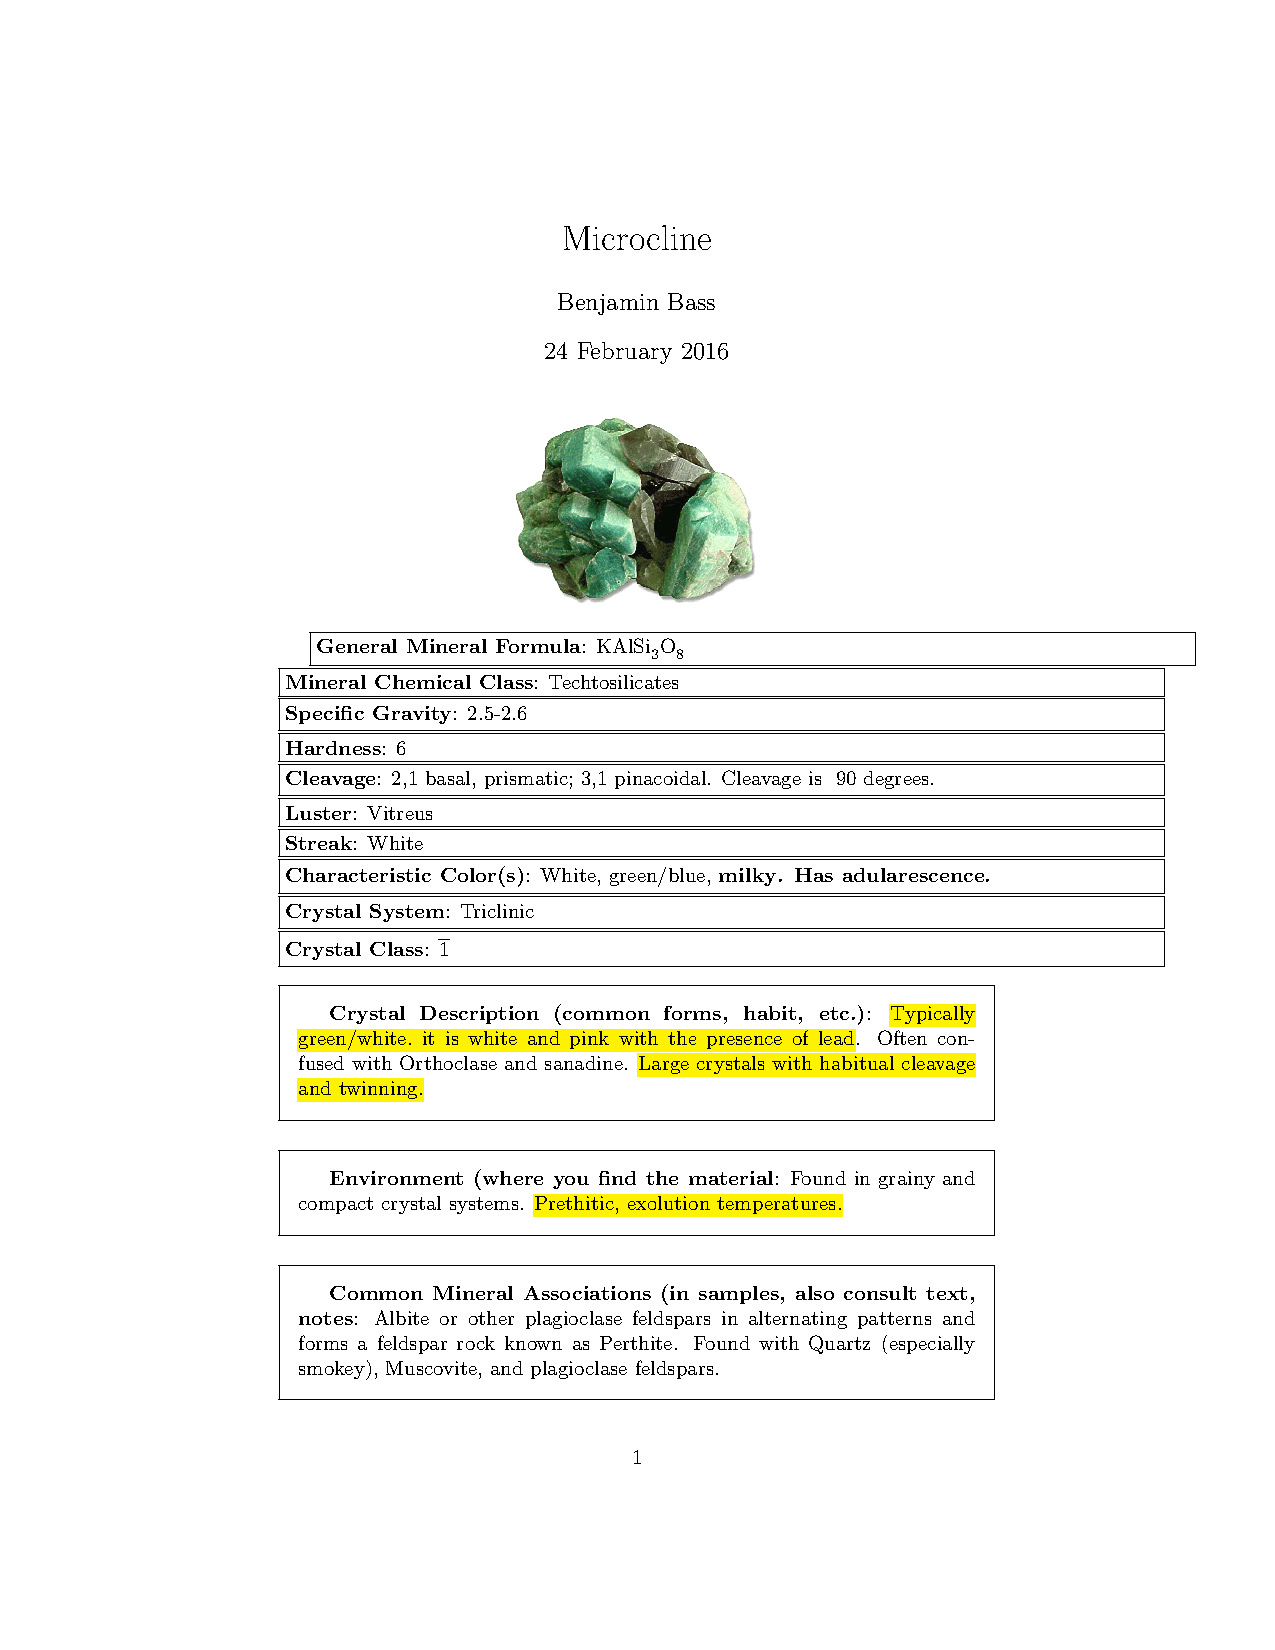
\includegraphics[scale=.25]{microcline}
\end{center}



\framebox[15cm][l]{\textbf{General Mineral Formula}: \ce{KAlSi3O8} }\
\framebox[15cm][l]{\textbf{Mineral Chemical Class}: Techtosilicates }\
\framebox[15cm][l]{\textbf{Specific Gravity}: 2.5-2.6 }\
\framebox[15cm][l]{\textbf{Hardness}: 6 }\
\framebox[15cm][l]{\textbf{Cleavage}: 2,1 basal, prismatic; 3,1 pinacoidal. Cleavage is ~90 degrees. }\
\framebox[15cm][l]{\textbf{Luster}: Vitreus }\
\framebox[15cm][l]{\textbf{Streak}: White }\
\framebox[15cm][l]{\textbf{Characteristic Color(s)}: White, green/blue, \bf{milky}. Has adularescence. }\
\framebox[15cm][l]{\textbf{Crystal System}: Triclinic  }\
\framebox[15cm][l]{\textbf{Crystal Class}: $\overline{1}$ }\

\begin{framed}
  \textbf{Crystal Description (common forms, habit, etc.)}: \hl{Typically green/white. it is white and pink with the presence of lead}. Often confused with Orthoclase and sanadine. \hl{Large crystals with habitual cleavage and twinning.}
\end{framed}

\begin{framed}
  \textbf{Environment (where you find the material}: Found in grainy and compact crystal systems. \hl{Prethitic, exolution temperatures.}
\end{framed}

\begin{framed}
  \textbf{Common Mineral Associations (in samples, also consult text, notes}: Albite or other plagioclase feldspars in alternating patterns and forms a feldspar rock known as Perthite. Found with Quartz (especially smokey), Muscovite, and plagioclase feldspars.
\end{framed}

\begin{framed}
  \textbf{Scientific Usage/Significance}: None
\end{framed}

\begin{framed}
  \textbf{Industrial or Social Use/Significance}: Important for the manufacture of glass and ceramics. A gemstone and often polished into beads.
\end{framed}

\begin{framed}
  \textbf{Environmental Significance}: Fairly stable in the weathering environment, it is a common constituent of detrital sedementary rocks.
\end{framed}

% Possible other Solutions
% \framebox(300,20){\minibox{\textbf{R-Sq}:For example}}

\end{document}
%%% Local Variables:
%%% mode: latex
%%% TeX-master: t
%%% End:
